\chapter{Background reading for users of MLS data}
\label{chap:Background}

\section{Aura MLS radiance observations}
\label{sec:MLSRadiances}

\begin{sidewaysfigure}
  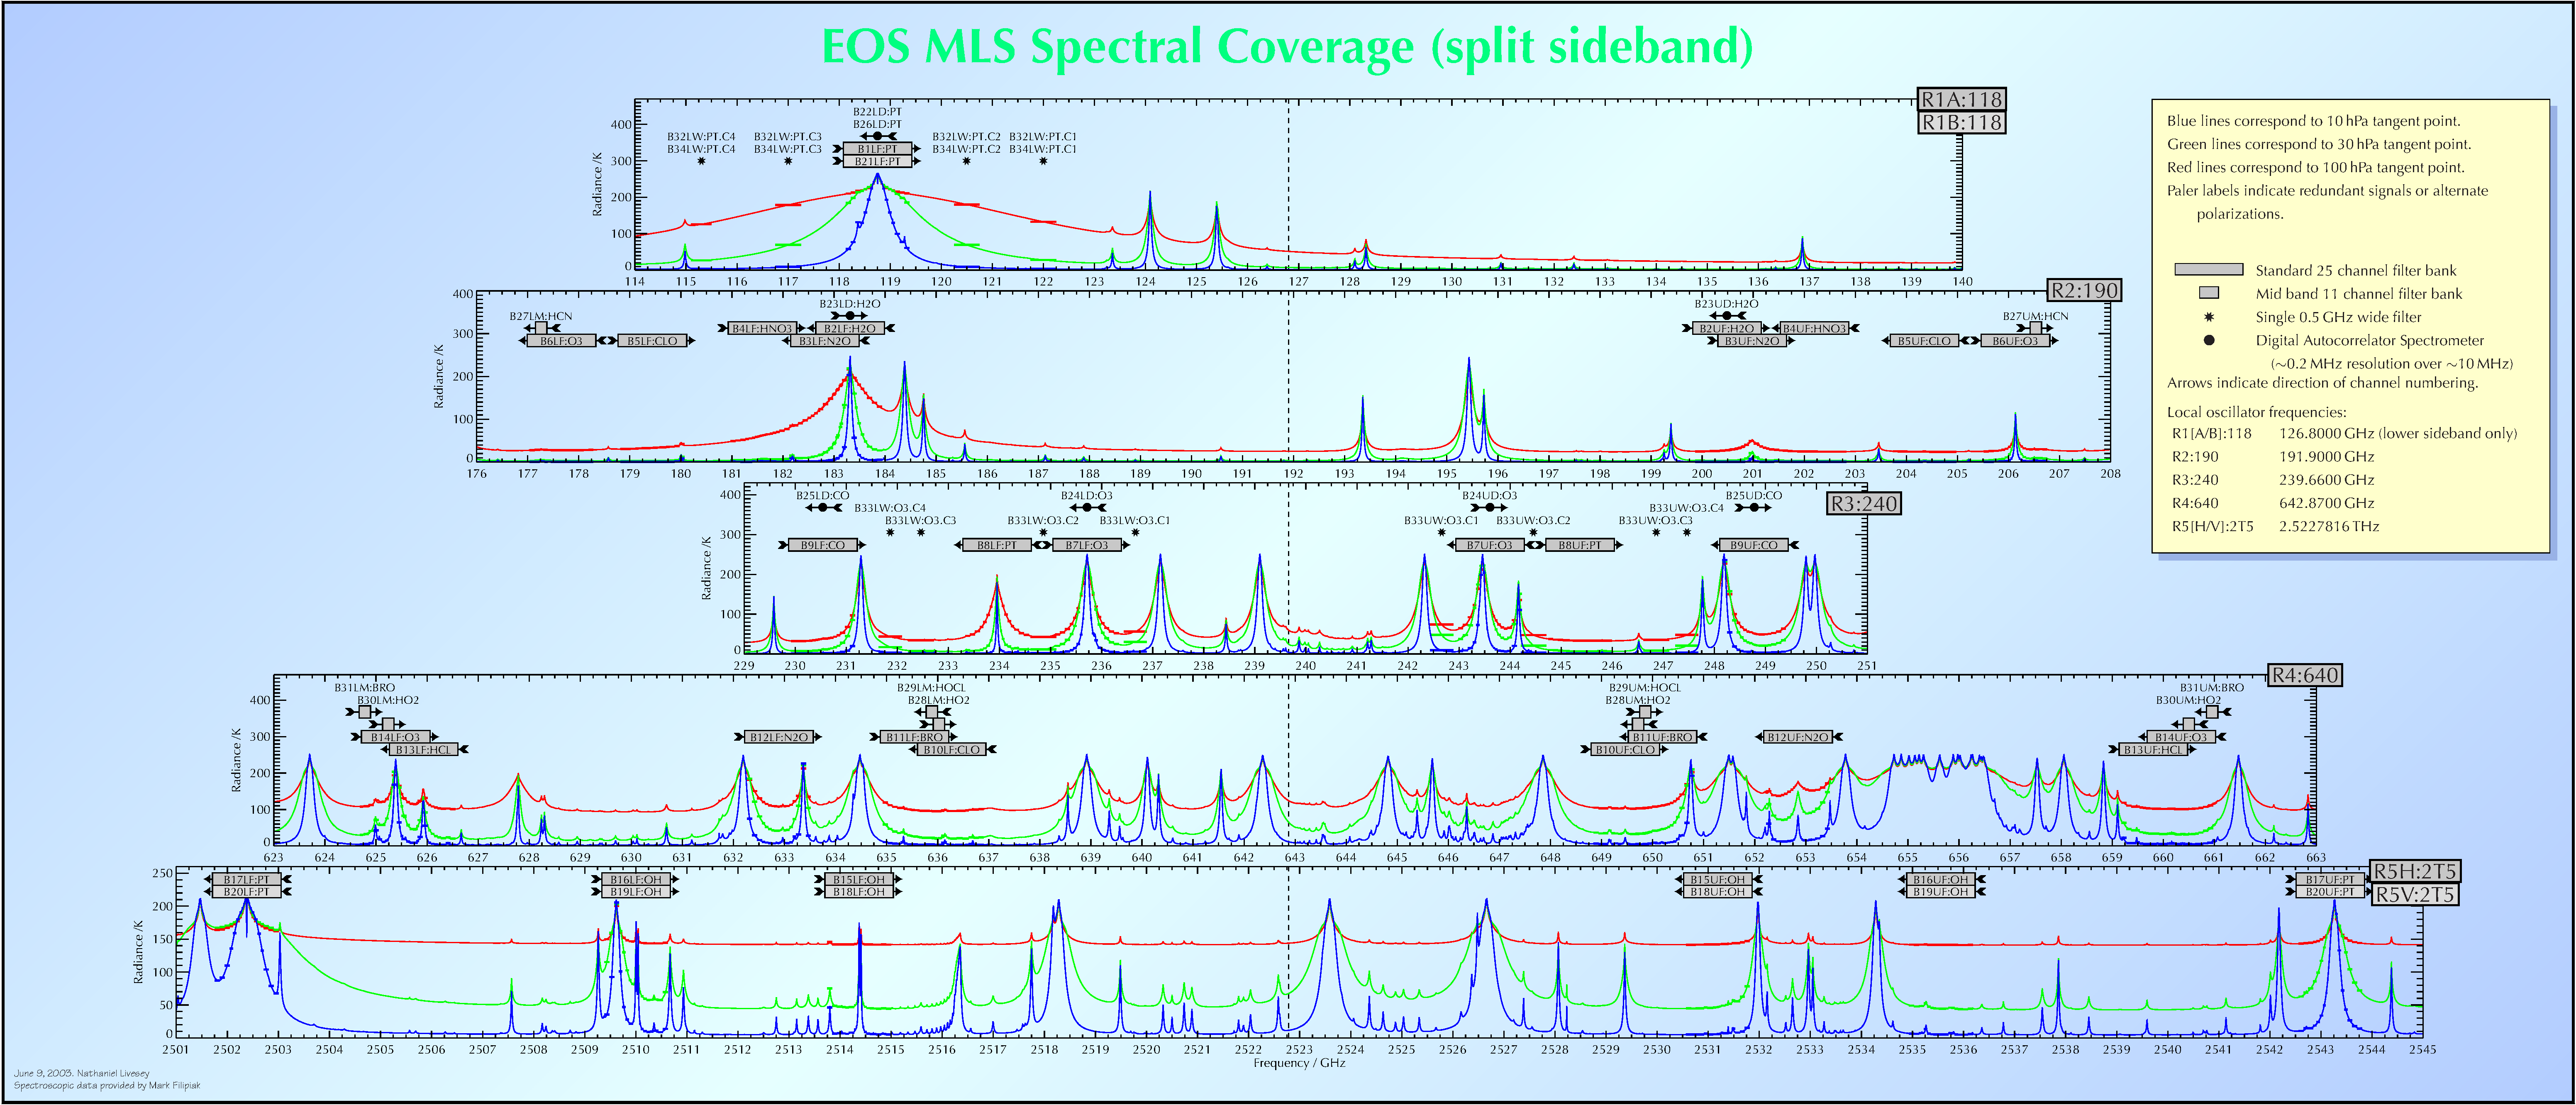
\includegraphics[width=\linewidth]{figures/unfolded-complete}
  \caption{The five panels show the spectral regions covered by the MLS radiometers.  The gray boxes and other symbols denote the position of the various ``bands'' observed within the spectral regions covered by each radiometer.}
  \label{fig:UnfoldedSpectra}
\end{sidewaysfigure}

\begin{figure}[htb]
  \includegraphics[width=\linewidth]{figures/folded-complete}
  \caption{This is similar to figure~\protect{\ref{fig:UnfoldedSpectra}}, except that x-axes represent ``intermediate frequency'' (IF).  The signal at each intermediate frequency represents a sum of the signals observed at that frequency both above (the ``upper sideband'') and below (the ``lower sideband'') the local oscillator. In the case of the \mbox{118-GHz} receivers, the upper sideband signals are suppressed, giving a single-sideband IF signal.)}
  \label{fig:FoldedSpectra}
\end{figure}

Figures~\ref{fig:UnfoldedSpectra} and~\ref{fig:FoldedSpectra} show the spectral coverage of the MLS instrument. The instrument consists of seven radiometers observing emission in the 118\nobreakdash-GHz (``R1A'' and ``R1B''), 190\nobreakdash-GHz (``R2''), 240\nobreakdash-GHz (``R3''), 640\nobreakdash-GHz (``R4'') and 2.5-THz (``R5H'' and ``R5V'') regions. With the exception of the two 118\nobreakdash-GHz devices, these are ``double sideband'' radiometers. This means that the observations from both above and below the local oscillator frequencies are combined and downconverted to form a \mytexttilde20\nobreakdash-GHz-bandwidth ``intermediate frequency'' signal. In the case of the 118\nobreakdash-GHz radiometers (R1A and R1B), the signals from the upper sideband (those frequencies above the \mytexttilde126\nobreakdash-GHz local oscillator) are suppressed. These intermediate frequency signals are then split into separate ``bands''. The radiance levels within these bands are quantified by various spectrometers.

In operation, the instrument performs a continuous vertical scan of both the GHz antenna (for R1A, R1B, R2, R3, and R4) and THz antenna (for R5H and R5V) from the surface to about 90\,km in a period of about 20\,s. This is followed by about 5\,s of antenna retrace and calibration activity. This \mytexttilde25\,s cycle is known as a \emph{major frame} (MAF). During the \mytexttilde20\,s continuous scan, radiances are reported at  \mytexttilde1/6\,s intervals, known as \emph{minor frames} (MIFs).  The scan timing is adjusted (through introduction of occasional ``Leap MIFs'' in selected MAFs) such that MLS performs exactly 240 scans during each orbit, with the latitudinal distribution of the scans being consistent from orbit to orbit. 

\section{Brief review of the theoretical basis}
\label{sec:TheoreticalBasis}

\begin{figure}[htb]
  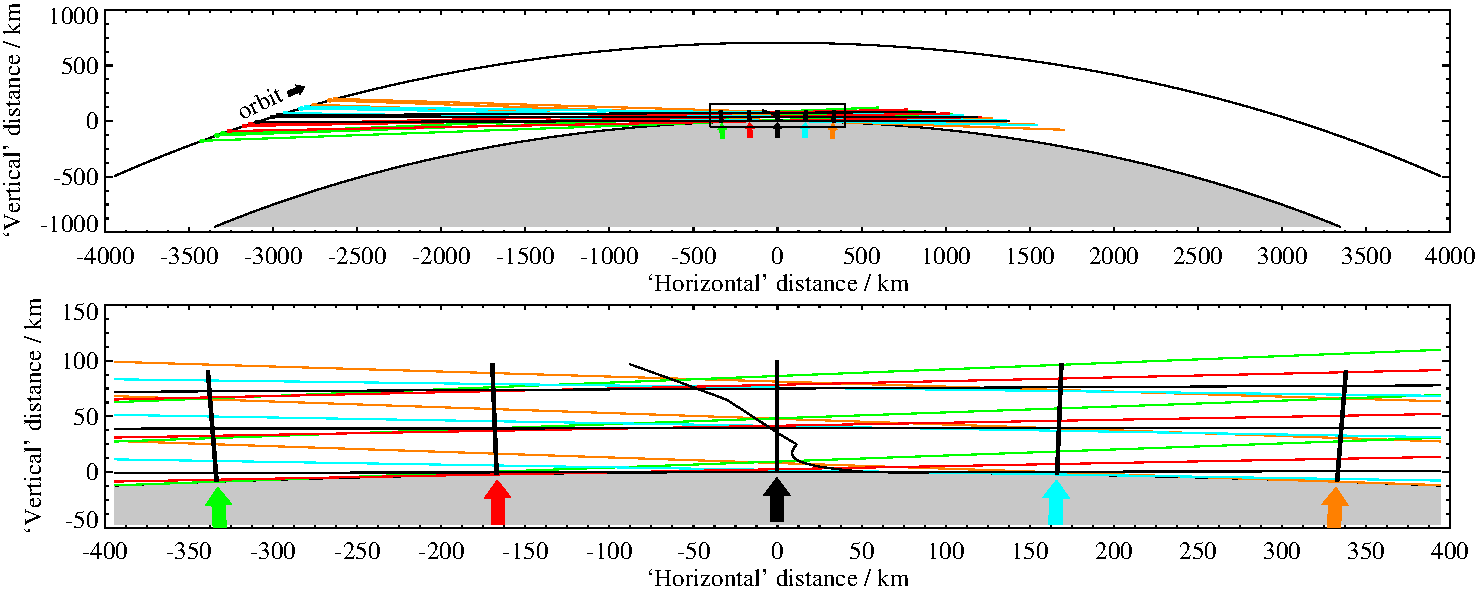
\includegraphics[width=\linewidth]{figures/geometry}
  \caption{The top diagram shows a section of one orbit.  Three of the 120 limb ray paths per scan are indicated by the ``horizontal'' lines.  The lower diagram shows an expansion of the boxed region above.  The straight radial lines denote the location of the retrieved atmospheric profiles.  The limb ray scan closest to each profile is that whose color is the same as that of the arrow underneath.  The thin black line under the central profile indicates the locus of the limb tangent point for this scan, including the effects of refraction.}
  \label{fig:Geometry}
\end{figure}

The Level~2 algorithms implement a standard \emph{Optimal Estimation} retrieval approach \citep{Rodgers:1976,Rodgers:2000} that seeks the ``best'' value for the ``state vector'' (the profiles of temperature and abundances) based on an optimal combination of the fit to the MLS radiance observations, a priori estimates of the state vector (from climatological information and, for temperature in the troposphere and lower stratosphere, analysis fields), and constraints on the smoothness of the result. This fit must often be arrived at in an iterative manner because of the non-linear nature of the Aura MLS measurement system.

An innovative aspect of the retrieval algorithms for Aura MLS \citep{LiveseyAndRead:2000, LiveseyEtal:2006} arises from taking advantage of the fact that the MLS instrument looks in the forward direction from the spacecraft. Figure~\ref{fig:Geometry} reviews the Aura MLS measurement geometry and shows that each radiance observation is influenced by the state of the atmosphere for several consecutive profiles. In the \thisv Level~2 algorithms, as with earlier versions, the state vector consists of ``chunks'' of several profiles of atmospheric temperature and composition, which are then simultaneously retrieved from radiances measured in a similar number of MLS scans. Results from these chunks are joined together to give products at a granularity of one day (the chunks overlap in order to avoid edge effects).

The retrieval state vector consists of vertical profiles of temperature and composition on fixed pressure surfaces. Between these fixed surfaces, the retrieval algorithms (more specifically the ``forward models'' within the retrieval system, see below) assume that species abundances and temperature vary from surface to surface in a piecewise-linear fashion (except for the abundance of \ch{H2O}, which is assumed to vary linearly in the logarithm of the mixing ratio). This has important implications for the interpretation of the data, as was described in Section~\ref{sec:BasisIssues}. In addition to these profiles, the pressure at the tangent point for the mid-point of each minor frame is retrieved, based on both radiance observations and knowledge of tangent point height, the latter computed from the MLS antenna position encoder readout and Aura spacecraft ephemeris and attitude information.

Most of the MLS data products are deduced from observations of spectral contrast, that is, variations in radiance as a function of frequency for a given limb pointing. Many of the systematic errors in the MLS measurement system manifest themselves as a spectrally flat or slowly spectrally varying error in radiance. This is true of effects arising both from the instrument (such as gain and offset during the limb scan) and from the ``forward model'' (such as knowledge of continuum emission and the impact of some approximations made in the forward model in order to increase its speed). In order to account for such effects, the \thisv algorithms also retrieve spectrally flat (or slowly spectrally varying) corrections to the MLS radiances, either in terms of an additive radiance offset or an additive atmospheric extinction.

\section{The ``Core, Core-plus-Rn\ldots'' approach to the MLS retrievals}

\subsection{The need for separate ``phases''}

Many aspects of the MLS measurement system are close to being linear in nature. In other words, there is a near-linear relationship between changes in aspects of the atmospheric state and consequent changes in the MLS radiance observations. However, there are some components of the state vector whose impact on the radiances is non-linear. The most non-linear components are the limb-tangent-point pressures for each MIF. The impact of water vapor in the upper troposphere on the MLS radiance observations is also highly non-linear. Solving for these aspects of the state vector therefore requires several iterations.  The computational effort involved in retrieval and forward models scales very rapidly (arguably as high as cubically) as a function of the size of the measurement system (i.e., the number of elements in the state and measurement vectors). Thus, it is desirable to simplify retrievals involving strongly non-linear variables to a small subset of the complete system, in order to cut down on the effort involved in retrievals that require many iterations.  Given those considerations, most remote-sounding retrieval algorithms are split into \emph{phases}. In the case of the MLS \thisv retrievals, there are many such phases. The first group of phases (collectively known as ``Core'') uses the 118\nobreakdash-GHz and 240\nobreakdash-GHz observations of O\cs2 and O\cp{18}O, respectively, to establish estimates for temperature and tangent pressure. Upper tropospheric 190\nobreakdash-GHz radiances are used in these early phases to establish a first-order estimate of upper tropospheric humidity. The Core phases also include cloud screening computations (based on differences between observed and estimated clear-sky radiances). These identify minor frames where radiances in a given radiometer have been subject to significant (and poorly modeled) cloud scattering. Such minor frames are ignored in \thisv processing of measurements from certain radiometers.

The Core phases are followed by phases such as \texttt{CorePlusR3} and \texttt{CorePlusR5}, where composition profiles are retrieved from a given radiometer. Sometimes (e.g., for \texttt{CorePlusR3}) these later phases continue to retrieve temperature and pressure, still using information from the 118\nobreakdash-GHz radiometers, as in the Core phases. In other phases (e.g., the \texttt{CorePlusR2} and \texttt{CorePlusR4} families of phases), the 118\nobreakdash-GHz information is neglected and temperature and pressure are constrained to the results from the earlier Core phases. This choice is made based on extensive testing aimed at maximizing the information yield from MLS while minimizing the impact of inevitable systematic disagreements among the different radiometers, introduced by uncertain spectroscopy and/or calibration knowledge.

Table~\ref{tab:Phases} describes the phases in more detail. Many products (e.g., ozone) are produced in more than one phase. All the separate measurements of these species are produced as diagnostic quantities, typically labeled according to the spectral region from which they originated. For example, the ozone product obtained from the \texttt{CorePlusR2} retrieval is known in the \thisv dataset as \texttt{O3-190}. In \thisv, as with previous versions, in order to reduce confusion for users of MLS data, the algorithms also output ``standard products'', which are typically copies of one of the products from the \texttt{CorePlusR\emph{n}} phases. For example, the standard chlorine monoxide product is a copy of the \texttt{ClO-640} product. In the case of \thisv nitric acid, the standard product represents a hybrid of the results from two phases. Details of which standard product is obtained from which phase are given in Table~\ref{tab:StandardProducts}. \mycomment{Talk to Frank about how to add cloud-top-pressure to the tables.}

\newcommand{\mybox}[2]{\parbox[m]{#1}{\raggedright #2}} \newcommand{\phase}[1]{\mybox{1.0in}{\texttt{#1}}} \newcommand{\species}[1]{\mybox{2.2in}{#1}} \newcommand{\measurements}[1]{\mybox{1.5in}{#1}} \newcommand{\tablecomments}[1]{\mybox{3.6in}{#1}}

\begin{sidewaystable}
  \renewcommand{\thempfootnote}{\sffamily[\arabic{mpfootnote}]}
  \renewcommand{\arraystretch}{1.2}
  \caption{The phases that form the \thisv retrieval
    algorithms.}  \vspace{1ex}
  \label{tab:Phases}
  \begin{minipage}{\linewidth}
    \begin{center}\begin{small}\sffamily
        \centering\begin{tabular}{llll}
        \rowcolor{tableheadbackground}
\tableheadentry{Phase} &
\tableheadentry{Target species\footnote{\sffamily Tangent pressure and Geopotential height have been abbreviated to pTan (GHz/THz) and GPH respectively.  Minor state vector components such as ``baseline'' and/or ``extinction'' have been omitted unless they are the specific focus of the phase.  Temperature, IWC, \ch{H2O}, RHi are ``high resolution'' (12 surfaces per decade change in pressure from 1000\,hPa to 1\,hPa) unless otherwise stated. \ch{O3} is low resolution except for the Core+R3 phase.}} &
\tableheadentry{Measurements} &
\tableheadentry{Comment} \\
\flipfloprow
\phase{InitPTan} &
\species{T, pTan (GHz), GPH} & 
\measurements{R1A \& R1B~(118\,GHz)} & 
\tablecomments{Initial estimate of P/T, lower limit 261\,hPa} \\

\flipfloprow
\phase{InitR2} &
\species{\ch{H2O}, \ch{N2O}, \ch{CH3CN}, HCN, ClO, \ch{HNO3}, \ch{O3}, SO\cs2} &
\measurements{R2~(190\,GHz)} &
\tablecomments{Initial trace gas estimator, lower limit 100\,hPa} \\

\flipfloprow
\phase{R3InitRHi} &
\species{RHi, T\cs{cir}} &
\measurements{R3 (240\,GHz)} &
\tablecomments{Retrieves RHi profile from 316\,hPa and up, used mostly
  for ``near field'' cloud detection and to compute R3 T\cs{cir}} \\

\flipfloprow
\phase{CloudDetector} &
\species{none} &
\measurements{R3 (240\,GHz)} &
\tablecomments{Determines cloud impacted radiance usage for R2 (190\,GHz), R3
  (240\,GHz) and R4 (640\,GHz)} \\

\flipfloprow
\phase{FinalPTan} &
\species{T, pTan~(GHz), GPH} & 
\measurements{R1A \& R1B~(118\,GHz), R3~(240\,GHz)} &
\tablecomments{Best P/T retrieval, lower limit 261\,hPa} \\ 

\flipfloprow
\phase{InitLowCloud} &
\species{T\cs{cir}} &
\measurements{All radiometers} &
\tablecomments{Computes cloud-induced radiance terms (T\cs{cir})} \\

\flipfloprow
\phase{InitRHi} &
\species{UT RHi} &
\measurements{R2~(190\,GHz)} &
\tablecomments{Retrieve RHi in a \mytexttilde6\,km-layer centered
  400--600\,hPa.  Uses only saturated radiances} \\ 

\flipfloprow
\phase{InitUTH} &
\species{Upper tropospheric \ch{H2O}} & 
\measurements{R2~(190\,GHz)} &
\tablecomments{Low vertical resolution (6/decade) \ch{H2O} retrieval} \\ 

\flipfloprow
\phase{CorePlusR3} & \species{T, pTan~(GHz), GPH, \ch{O3}\footnote{\sffamily On high vertical resolution grid}, CO, \ch{HNO3}, SO\cs2, RHi} &
\measurements{R1A \& R1B~(118\,GHz), R3~(240\,GHz)} &
\tablecomments{Retrievals down to 316\,hPa}\\ 

\flipfloprow
\phase{OzoneOnly} &
\species{\ch{O3}, CO} &
\measurements{R3~(240\,GHz)} &
\tablecomments{Retrievals down to 316\,hPa optimized for \ch{O3} product}\\ 

\flipfloprow
\phase{CorePlusR2} &
\species{\ch{H2O}, \ch{N2O}, \ch{HNO3}, ClO, \ch{O3}, HCN, \ch{CH3CN}, SO\cs2, pTan~(GHz)} &
\measurements{R1A \& R1B~(118\,GHz), R2~(190\,GHz)} & 
\tablecomments{\ch{H2O} retrieved down to 316\,hPa, other species 100\,hPa (note no T, GPH, pTan retrieval)} \\ 

\flipfloprow
\phase{Hydrogen Cyanide} &
\species{HCN, \ch{O3}, \ch{HNO3}} &
\measurements{R2~(190\,GHz)} & 
\tablecomments{Retrievals down to 100\,hPa} \\ 

\flipfloprow
\phase{CorePlusR4AB14} & \species{ClO, BrO, \ch{HO2}, HOCl,
  HCl, \ch{O3}, \ch{HNO3}, \ch{CH3CN}, SO\cs2, \ch{CH3Cl}} &
\measurements{R4~(640\,GHz)} &
\tablecomments{Retrievals down to 147\,hPa}\\ 

\flipfloprow
\phase{Methanol} &
\species{\ch{CH3OH}, ClO, BrO, \ch{HO2}, HOCl, \ch{HNO3}, SO\cs2, \ch{CH3Cl}} &
\measurements{R2~(190\,GHz) and R4~(640\,GHz)} & 
\tablecomments{Retrievals down to 147\,hPa} \\ 

\flipfloprow
\phase{CorePlusR4AB13} & \species{HCl, \ch{O3}, SO\cs2} &
\measurements{R4~(640\,GHz)} &
\tablecomments{Retrievals down to 147\,hPa. This phase is only executed when
  MLS band~13 is operating}\\ 

\flipfloprow
\phase{CorePlusR4B} & \species{\ch{N2O}, SO\cs2} &
\measurements{R4~(640\,GHz)} &
\tablecomments{Retrievals down to 147\,hPa. This phase is only executed when MLS band~12 is operating}\\ 

\flipfloprow
\phase{HighCloud} &
\species{Cloud induced radiance, IWC, IWP} &
--- &
\tablecomments{Generates cloud ice (IWC, IWP) products} \\ 

\flipfloprow
\phase{CorePlusR5} & \species{T, pTan~(GHz,~THz), GPH, OH, \ch{O3}} &
\measurements{R1A \& R1B~(118\,GHz), R5H and R5V~(2.5\,THz)} &
\tablecomments{Retrievals down to 68\,hPa (147\,hPa for Temperature). This phase is only executed when the MLS THz module is operating} \\

\flipfloprow
\phase{GPHOnly} & \species{GPH} & --- &
\tablecomments{Offsets CorePlusR3 GPH to match GEOS-5 at 100\,hPa}\\

\end{tabular}
      \end{small}\end{center}
  \end{minipage}
\end{sidewaystable}

\begin{table}
  \sffamily
  \renewcommand{\arraystretch}{1.3}
  \caption{The origin of each of the ``standard products'' from
    \thisv.}
  \vspace{1ex}
  \label{tab:StandardProducts}
  \centering\begin{tabular}{l>{\ttfamily}ll}
  \rowcolor{tableheadbackground}
  \tableheadentry{Product} & \sffamily\tableheadentry{Origin} & \tableheadentry{Spectral region}\\
  \flipfloprow
  BrO       & CorePlusR4AB14 & 640\,GHz \\
  \flipfloprow 
  \ch{CH3Cl}  & CorePlusR4AB14 & 640\,GHz \\
  \flipfloprow 
  \ch{CH3CN}  & CorePlusR4AB14 & 640\,GHz \\
  \flipfloprow 
  \ch{CH3OH}  & Methanol & 640\,GHz \\
  \flipfloprow 
  ClO       & CorePlusR4AB14 & 640\,GHz \\
  \flipfloprow 
  CO        & CorePlusR3 & 240\,GHz \\
  \flipfloprow 
  GPH       & GPHOnly & 118 \& 240\,GHz \\
  \flipfloprow 
  \ch{H2O}    & CorePlusR2 & 190\,GHz \\
  \flipfloprow 
  HCl       & CorePlusR4AB14 & 640\,GHz \\
  \flipfloprow 
  HCN       & HydrogenCyanide & 190\,GHz \\ 
  \flipfloprow 
  \ch{HNO3}   & \mybox{6cm}{CorePlusR2 \textsf{(15\,hPa and less)} \\ CorePlusR3 \textsf{(larger
    than 15\,hPa)}} &
  \mybox{2.5cm}{190\,GHz\\240\,GHz} \\
  \flipfloprow 
  \ch{HO2}    & CorePlusR4AB14 & 640\,GHz \\
  \flipfloprow 
  HOCl      & CorePlusR4AB14 & 640\,GHz \\
  \flipfloprow 
  IWC       & HighCloud & 240\,GHz \\
  \flipfloprow 
  IWP       & HighCloud & 240\,GHz \\
  \flipfloprow 
  \ch{N2O}    & CorePlusR2 & 190\,GHz \\ 
  \flipfloprow 
  \ch{O3}     & OzoneOnly & 240\,GHz \\
  \flipfloprow 
  OH        & CorePlusR5 & 2.5\,THz \\
  \flipfloprow 
  RHi       & \mybox{6cm}{\sffamily\raggedright Computed from Temperature and \ch{H2O}} & 190\,GHz \\
  \flipfloprow 
  SO\cs2    & CorePlusR3 & 240\,GHz \\
  \flipfloprow 
  Temperature & CorePlusR3 & 118 \& 240\,GHz \\
\end{tabular}
\end{table}

\section{MLS forward models}

At the heart of any optimal-estimation-based retrieval lies one or more ``forward models''.  These are tasked with computing estimates of the radiances the instrument would measure when viewing an atmosphere described by a given state vector.  The retrieval iteratively updates this state vector such that the corresponding forward model radiances agree satisfactorily with the measured radiances.   The state vector updates made each iteration are driven by the ``Jacobian'' information (the derivative of the predicted radiance with respect to the estimated state, also known as ``weighting functions'') that is also computed by the forward model.  The retrieval algorithms in \thisv make use of a variety of different forward models. The most accurate is the so-called ``full forward model'' described in \citet{EOSMLSFWMATBD} and \citet{EOSMLSPolarizedFWMATBD}. This is a hybrid line-by-line and channel-averaged model that computes radiances on appropriate grids of frequency and limb tangent pressure that are then convolved with the MLS frequency and angular responses.  This model is generally rather time consuming, although for some comparatively ``clean'' spectral regions the computational burden is small enough that the full forward model was used in early versions of the operational retrievals. In the years since the Aura launch, computational capabilities have improved significantly, enabling use of the full forward model for all MLS channels in more recent MLS data versions.

For some of the MLS channels, a simpler ``linearized forward model'' can be used to estimate radiances, or more typically just the Jacobian information, with the radiances still being computed by the full forward model. The linearized model invokes a simple first-order Taylor series to estimate radiances as a function of the deviation of the state from one of several pre-selected representative states. The inputs to this model are pre-computed radiances and derivatives corresponding to the pre-selected states, generated by stand-alone runs of the full forward model.

In addition, a ``cloud forward model'' can be invoked to model the effects of scattering from cloud particles in the troposphere and lower stratosphere \citep{EOSMLSCloudATBD}. This model was used in the simulation of radiances based on known model atmospheres for the \thisv testing but is not invoked in the \thisv retrieval algorithms, as discussed below.

\section{The handling of clouds in MLS retrievals}
\label{sec:Clouds}
\newcommand{\Tcir}{\ensuremath{T_\text{cir}}}

While MLS observations are insensitive to aerosols and thin clouds, the particle sizes and number densities associated with strong deep convective clouds can lead to scattering of the signals at the millimeter-scale wavelengths observed by MLS.  Broadly speaking, this scattering redirects some fraction of the ambient radiation in the cloudy region towards the MLS antenna. This ambient radiation will be a mix of ``bright'' upwelling radiances and ``dark'' signals downwelling from cold space. Thus, for high-altitude optically thin limb views, where small radiance signals are seen in cloud-free situations, cloud scattering will increase the observed radiances. On the other hand, for low-altitude limb views, characterized by large radiances in cloud-free scenes, clouds in the line-of-sight will act to suppress the observed radiances, as some of the observed signal will originate from downwelling signatures of cold space scattered into the beam.

The MLS \thisv algorithms can reliably retrieve composition in moderately cloudy cases (i.e., those having small limb radiance perturbations).  In the case of the \texttt{CorePlusR3} retrieval this is handled by retrieving a frequency-squared-dependent extinction (including background atmospheric absorption from N\cs2, \ch{H2O}, and unknown emitters). In the other retrieval phases, by contrast, a spectrally flat radiance baseline term is used. Thick clouds can affect the MLS radiances beyond the modeling capability of this approach, mainly through scattering processes. In such situations, the affected radiances are excluded from the retrievals, or their influence is down-weighted.

The first aspect of handling clouds in \thisv is therefore the flagging of radiances that are believed to be significantly contaminated by cloud effects.   In the \texttt{CorePlusR2}, \texttt{CorePlusR3}, and \texttt{CorePlusR4[\ldots]/\texttt{Methanol}} phases, cloud flagging is based on determining the highest-altitude limb view contaminated by cloud signals and rejecting all radiances below that targeted altitude.  Cloud radiance scattering narrows the line shape for any molecule.  The O\cp{18}O line measured by MLS ``Band~8'' is a convenient signal to use for cloud detection as (1) the concentration of O\cp{18}O is well known, (2) its signal is at a relatively high frequency, making it more susceptible to cloud scattering effects than many (but not all) other MLS signals, and (3) the line never goes opaque at any altitude, making it sensitive to tangent pressure into the upper troposphere.

The detection of cloud scattering is based on a poor lineshape fit (typically manifested as the measured linewidth being unphysically narrow compared to the calculated width).  The calculation uses estimates of tangent pressure and temperature obtained from the 118\nobreakdash-GHz Band~1 measurements (unaffected by clouds) and tangent point altitude information obtained from instrument/spacecraft pointing knowledge. These, combined with an estimate of relative humidity from a previous retrieval phase, are used to compute the radiances expected in a clear-sky scene.  These are compared to the measured \mbox{Band-8} radiances to give estimated cloud-induced radiances (\Tcir). The vertical profiles of a $\chi^2$ parameter and \Tcir\ are analyzed to find the highest limb view affected by cloud scattering, and radiances below are handled accordingly. \mycomment{Get Bill to read this again.}

The other aspect of cloud handling in \thisv is the estimation of cloud ice water content (IWC) and ice water path (IWP) products from the final \Tcir\ computed by the retrieval in the \texttt{HighCloud} phase. More information on these products and their derivation is given in Sections~\ref{sec:StandardIWC} and~\ref{sec:StandardIWP}.  For details of a cloud top pressure product that is new in \thisv, see Section~\ref{sec:StandardCldTopP}.

\begin{table}
  \sffamily%\mathversion{sans}
  \renewcommand{\arraystretch}{1.4}
  \caption{MLS frequency channels and thresholds for the cloud flag.}
  \vspace{1ex}
  \label{tab:CloudThresholds}
  \centering\small\begin{tabular}{>{\ttfamily}l>{\ttfamily}llll}
  \rowcolor{tableheadbackground}
  \sffamily\tableheadentry{Radiometer} &
  \sffamily\tableheadentry{Cloud channel} &
  \tableheadentry{USB/LSB frequency / GHz} & 
  \tableheadentry{Low threshold} & \tableheadentry{High threshold} \\
%
\flipfloprow
R1A:118 & B32W:PT.C4 & 115.3 (LSB only) & 
$\mathsf{\Tcir < -4}$\,K &
 none \\
%
\flipfloprow
R1B:118 & B34W:PT.C4 & 115.3 (LSB only) & 
$\mathsf{\Tcir < -4}$\,K &
none \\
%
\flipfloprow
R2:190 & B5F:ClO.C1 & 178.8 / 204.9 &
$\mathsf{\Tcir < -20}$\,K &
$\mathsf{\Tcir > 10}$\,K \\
%
\flipfloprow
R3:240 & B8F:PT & 233.4--234.5 / 244.8--245.9 & none &
$\mathsf{\chi^2>30}$ \\
%
\flipfloprow
R4:640 & B11F:BrO.C23 & 635.9 / 649.8 & 
$\mathsf{\Tcir < -10}$\,K &
none \\
\end{tabular}
\end{table}

\section{The quantification of systematic uncertainty in MLS data}
\label{sec:SystematicUncertainty}

A major component of the validation of MLS data is the quantification of the various sources of systematic uncertainty. These can arise from instrumental issues (e.g., radiometric calibration, field of view characterization), spectroscopic uncertainty, and approximations in the retrieval formulation and implementation. Comprehensive quantification of these uncertainties has been performed for \thisv MLS products, updated from that described in the MLS validation papers (which were based on \vii). The individual sections of Chapter~\ref{chap:Level2} detail the results of this quantification for each product.

For each identified source of systematic uncertainty, its impact on MLS measurements of radiance (or pointing where appropriate) has been quantified and modeled. These modeled impacts correspond to either 2$\sigma$ estimates of uncertainties in the relevant parameter(s) or an estimate of their maximum reasonable error(s) based on instrument knowledge and/or design requirements. Accordingly, the numbers reported for each product in Chapter~\ref{chap:Level2} reflect 2$\sigma$ estimates of potential systematic error.

For most of the uncertainty sources, the impact on MLS standard products has been quantified by running perturbed radiances through the MLS data processing algorithms. Other (typically smaller) uncertainty sources have been quantified by simple perturbation calculations.

Although the term ``systematic uncertainty'' is often associated with consistent biases and/or scaling errors, many sources of ``systematic'' error in the MLS measurement system give rise to additional scatter. For example, an error in the ozone spectroscopy, while being a constant bias on the fundamental parameter, will have an impact on the retrievals of species with weaker signals (e.g., CO) that is dependent on the amount and morphology of atmospheric ozone. By performing end-to-end simulations of the impacts of systematic errors, it is possible to quantify the extent to which such uncertainties either ``cancel-out'' (e.g., a truly constant bias will not impact a trend calculation) or ``average down'' (e.g., the impact of ozone-spectroscopy-related errors in MLS CO may be reduced by averaging in some circumstances).  A comprehensive consideration of such issues is beyond the scope of most scientific investigations using MLS data.  However, first-order insights can be obtained by considering both the bias and the additional scatter each error source introduces. Accordingly, for each product, the results of the MLS systematic error quantification studies are summarized in Chapter~\ref{chap:Level2} as ``accuracy'', in some cases supplemented with an estimate of additional contributions to ``precision'' \mycomment{Check wording in tables}. More details on the accuracy quantification for each product are given in the respective \vii MLS validation papers. In addition, Appendix~A of \citet{ReadEtal:2007} gives more specific details of the perturbations used in those quantifications.

\section{A brief note on the \texttt{Quality} field}

As described in Section~\ref{sec:StatusQuality}, the \texttt{Quality} field in the \texttt{L2GP} files gives a measure of the fit achieved between the observed MLS radiances and those computed by the forward model given the retrieved MLS profiles. \texttt{Quality} is computed from a $\chi^2$ statistic for all the radiances considered to have significantly affected the retrieved species (i.e., those close to the relevant spectral lines), normalized by dividing by the number of radiances. \texttt{Quality} is simply the reciprocal of this statistic (a metric chosen such that low values of ``quality'', corresponding to large $\chi^2$, indicate poor fits).

Ideally, the typical values of these normalized $\chi^2$ statistics will be around one, indicating that radiances are typically fitted to around their noise levels. \texttt{Quality} will therefore also ideally have a typical value of one. For some species, however, because of uncertain knowledge of spectroscopy and/or instrument calibration, the \thisv algorithms are known to be consistently unable to fit some observed radiances to within their predicted noise. In many of these cases, the noise reported on the radiances has been ``inflated'' to allow the retrieval more leeway in fitting to radiances known to be challenging. As the noise level is the denominator in the $\chi^2$ statistic, these species will have typical $\chi^2$ statistics that are less than one and thus typical values of \texttt{Quality} higher than one. Accordingly, differences in \texttt{Quality} from one species to another do not reflect the species' relative validity, nor do version-to-version increases in \texttt{Quality} for a given product necessarily indicate improvements.

\section{Changes in \thisv retrievals of \texorpdfstring{\ch{N2O}}{N2O}}
\label{sec:V6N2OCorrectionDetails}

As discussed in Section~\ref{sec:V6N2OCorrectionBriefSummary}, in the \thisv algorithms changes were made to the manner in which \ch{N2O} is retrieved from radiances measured by the MLS 190\nobreakdash-GHz radiometer.  MLS observes \ch{N2O} by measuring a spectral line that (particularly in the folded-sideband MLS measurements) is spectrally close to, but 25 times weaker than, the \ch{H2O} line at 183\,GHz. The sideband fraction fix developed for the CorePlusR2 products in \prevv (see Sections~\ref{sec:StandardH2O} and~\ref{sec:StandardN2O}, as well as \citet{LiveseyEtal:2021:Drifts}) clearly improved \ch{H2O} (and \ch{O3} measurements made by the 190\nobreakdash-GHz radiometer) but, for unknown reasons, degraded \ch{N2O}. As an unsatisfying workaround for this issue, \ch{N2O} in \prevv was retrieved from a separate phase where the sideband fractions were based on the prelaunch calibration value (in contrast with \ch{H2O}, which was retrieved using a corrected value for this fraction), with a correction for the drift. This phase also unrealistically assumed no contribution to the 190\nobreakdash-GHz signals from continuum emission.  With the exception of drift correction, these changes were empirically derived and non-physical \citep{LiveseyEtal:2021:Drifts}.  For \thisv \ch{N2O} we opted to instead determine a correction for the 190\nobreakdash-GHz radiances based on \ch{N2O} information obtained from the stronger and less interference-prone 640\nobreakdash-GHz line (measurements from which were available from launch through August 2013). Using a subset of the days for which 640\nobreakdash-GHz \ch{N2O} measurements are available, we examined the spectral and scan-angle-dependent form of the correction needed to improve the agreement between the 190- and 640\nobreakdash-GHz \ch{N2O} products.  In order to reduce the dependence on specifics of the MLS scan etc., we opted to characterize the correction as a function of the total integrated radiance measured across the 190\nobreakdash-GHz band, as a proxy for limb tangent pressure and other parameters.  With this correction in place, a separate phase for retrieving \ch{N2O} is no longer needed, and the standard \ch{N2O} product is again retrieved concurrently with \ch{H2O} and \ch{HNO3} (for pressure $\le$ 14.7\,hPa) from the CorePlusR2 phase, as in \viv and previous versions. The root of the issue is that the interference between the strong \ch{H2O} line and the weak \ch{N2O} signature is not modeled well enough to provide an accurate \ch{N2O} retrieval (e.g., to within 10\%), especially in the lower stratosphere and upper troposphere.